%% LyX 2.0.8.1 created this file.  For more info, see http://www.lyx.org/.
%% Do not edit unless you really know what you are doing.
\documentclass[english]{article}
\usepackage[T1]{fontenc}
\usepackage[latin9]{inputenc}
\usepackage{graphicx}

\makeatletter

%%%%%%%%%%%%%%%%%%%%%%%%%%%%%% LyX specific LaTeX commands.
%% A simple dot to overcome graphicx limitations
\newcommand{\lyxdot}{.}


%%%%%%%%%%%%%%%%%%%%%%%%%%%%%% User specified LaTeX commands.
\usepackage{algorithm} % http://ctan.org/pkg/algorithms
\usepackage{algpseudocode}% http://ctan.org/pkg/algorithmicx    
\usepackage{mathtools}
\newcommand\tab[1][1cm]{\hspace*{#1}}

\makeatother

\usepackage{babel}
\begin{document}

\title{GAntenna Cover Algorithm}

\maketitle

\section*{Problem Statement}

Given the following:
\begin{itemize}
\item An unlimited supply of sensors, each of which can have multiple antennas,
such that :

\begin{itemize}
\item All antennas have the same aperture angle.
\item A sensor has at least one antenna.
\item A given sensor can have multiple antennas. 
\item Each antenna belonging to a given sensor has the same sensitivity
but each antenna assigned to a sensor may have a different roatation
(azimuth) angle.
\item Different sensors may have antennas having different sensitivities.
\item Sensors can each have different numbers of antennas.
\end{itemize}
\item A set of \textit{possible\_locations} in 2-d space where sensors may
be placed sorted in z-order (also known as Morton order). Call the
lines joining these points in order the \textit{Coastal Line} (CL).
\item An set of \textit{interference\_knot\_points} sorted in z-order. Call
the lines joining these points the \textit{Interference Contour} (IC).
\item CL and IC do not intersect.
\end{itemize}
We call the simple polygon constructed by adding edges from the extremities
of IC to CL, the \textit{Coverage Region} (CR). Our goal is to cover
CR such that:
\begin{itemize}
\item The the entire area of CR is covered to within a defined tolerance
(i.e. the tolerance is some small number < 1 denoting the fraction
of the area not covered by any antenna).
\item The region outside CR covered by the antennas is minimized. We call
this the \textit{Excess Region} (ER).
\item The total area of the cover (i.e. the sum of all the areas covered
by each antenna) is minimized.
\item No two sensors are closer to each other than some defined minimum
distance \textit{min\_distance}
\end{itemize}
Determine the following:
\begin{itemize}
\item Optimal placement of the sensors 
\item Orientation of the antennas (i.e. azimuth angle with respoect to the
horizontal). 
\item Calibration of the antennas (i.e. \textquotedbl{}optimum\textquotedbl{}
detection range of the antennas at each location where they are placed). 
\end{itemize}

\section*{Algorithm High Level Description}

\textbf{Inputs}: 
\begin{itemize}
\item The sorted set of \textit{possible\_centers}
\item The sorted set of \textit{interference\_knot\_points }
\item The \textit{min\_distance} specifying the minimum separation between
two sensors.
\item A family of concetric \textit{detection\_coverage} curves definining
the coverage regions for different antenna sensitivities all oriented
in the same direction. These antenna curves are closed convex curves
centered at \textit{(0,0)} that, in general do not pack into a circle
without overlap. 
\end{itemize}

\paragraph{Algorithm}
\begin{enumerate}
\item Construct the \textit{coverage\_region} (CR):

\begin{enumerate}
\item Constuct a multi-line segment consisting of the points in \textit{possible\_centers}
joined in order.
\item Construct a multi-line segment consisting of the \textit{interference\_knot\_points}
joined in order.
\item Complete the simple polygon to generate CR.
\end{enumerate}
\item Generate a rectangular grid of points such that each point of the
grid is entirely within the region CR. ( We start with some default
grid spacing. This may be adjusted in subsequent steps.) We call the
grid of points thus generated the \textit{interference\_set}.
\item Generate a greedy circle cover (isotropic antenna) for \textit{(possible\_centers,
interference\_set, minum\_separation) }using algorithm \textit{min\_area\_cover\_greedy}.
This returns a set of centers chosen from \textit{possible\_centers}
and a set of radii of circles that cover the\textit{ interference\_set}
such that antennas are spaced apart by at least \textit{min\_distance}
and the set of circles completely covers \textit{interference\_set}
\item Place the antenna lobes (chosen from \textit{detection\_coverage}
) within the circles returned from step 3 such that the antenna lobes
completely cover the intersection area between the circles and CR
using algorithm \textit{find\_antenna\_overlay\_for\_sector}. 
\item Using simulated annealing with a cost function defined as the area
of the convex hull of the cover, rotate the antenna cover lobes on
their assigned sensors so that the cost function is minimized.
\item Eliminate redundant antenna lobes.
\end{enumerate}
We now present the non-obvious steps in greater detail:


\begin{algorithm}[!htb] 
\caption{\textbf{$find\_max\_min\_circle$}: Find the center and radius of a circle with center $c$ and radius $r$ 
for $c$ $\in$ $possible\_centers$  and $p$  $\in$ $interference\_set$ such that 
a circle centered at $c$ covers $p$ and has maximal radius among all such circles.} 
\begin{algorithmic} 
\State \textbf{Parameters:} 
\State \tab  $possible\_centers$: The possible centers in the 2-dimensional plane 
\State \tab  where sensors may be placed sorted in z-order. 
\State \tab $interference\_set$: A set of points to be covered by cricles placed 
\State \tab \tab \tab at $possible\_centers$. 
\State \textbf{Output:} 
\State \tab $(c,r)$ where $c$ is the center coordinate of the circle to be placed and $r$ 
\State \tab is the radius of a circle placed at $c$.
\State \textbf{Procedure:} 
\State
\State $closest\_centers$ := \bf{select} ( \{ $(c,p,r)$ : $c$ $\in$ $possible\_centers$ 
\State \tab \tab \tab                       $\wedge$ $p$  $\in$ $interference\_set$ 
\State \tab \tab \tab                       $\wedge$ r = \bf{euclidean\_distance}($c$,$p$)
\State \tab \tab \tab                       $\wedge$ r is minimal \} )
\State $max\_min\_center$ := \bf{select} ( \{ $(c,p,r)$ :
\State \tab \tab \tab 				      $(c,p,r)$ $\in$ $closest\_centers$ 
\State \tab \tab \tab                     $\wedge$ $r$ is maximal \} )
\State \Return $(max\_min\_center.c,max\_min\_center.r)$ 
\end{algorithmic}
\end{algorithm}

\begin{algorithm}[!htb]
\caption{\textbf{$min\_area\_circle\_cover\_greedy$}: Find the greedy minimum area circle cover to cover a given $interference\_set$.}
\begin{algorithmic}
\State \textbf{Parameters:}
\State \tab $interference\_set$: Set of interference points that we want to cover
\State \tab $possible\_centers$: Set of possible centers.  
\State \tab $min\_distance$: Minimum distance permissible between circle centers. 
\State \textbf{Output:}
\State \tab $cover$ : A set of circles \{$(c,r)$ :  the circles completely 
\State \tab \tab cover $interference\_set$.\}
\State \textbf{Procedure:}
\State
\State $circle\_cover$ = $\emptyset$
\While { $interference\_set$ is not $\emptyset$ }
\State $(center,radius)$ := $find\_max\_min\_circle$ ( $interference\_set$, 
\State \tab \tab \tab $possible\_centers$ )
\State $covered\_points$ = \{ p : p $\in$ $interference\_set$ $\wedge$ p is inside circle(c,r) \}
\State // Check if this center already exists in our cover
\If {$\exists$ $(c,r_1)$ $\in$ $cover$ : c = $center$ }
\State  	$circle\_cover$ := $circle\_cover$ - \{$(c,r_1)$\} $\cup$ \{$(c,max(radius,r_1))$\}
\Else 
\State 	$circle\_cover$ := $circle\_cover$ $\cup$ $(center,radius)$
\EndIf
\For{k $\in$ $possible\_centers$} 
\State // Remove centers closer than $min\_distance$.
\If {\bf{euclidean\_distance}$(k,c)$ $\le$ $min\_distance$} 
\State $possible\_centers := possible\_centers - \{k\}$
\EndIf
\EndFor
\State // Prune the interference set.
\State $interference\_set$ := $interference\_set$ - $covered\_points$
\EndWhile
\State \Return $circle\_cover$
\end{algorithmic}
\end{algorithm}


\begin{algorithm}[!htb]
\caption{\textbf{$find\_antenna\_overlay\_for\_sector$} : Position the antenna lobes within a section bounded by a circle (which is part of the $circle\_cover$) and $coverage\_region$ }
\begin{algorithmic}
\State \textbf{Parameters:}
\State \tab $points\_to\_cover$ : A set of grid points that define the 
\State \tab \tab sector to be covered.
\State \tab $center$ : center of the circle that covers the sector.
\State \tab $radius$ : Radius of the circle that covers the sector.
\State \tab $detection\_coverage\_lobe$ : Antenna lobe of size 1.2*radius oriented 
\State \tab \tab in the horizontal direction. 1.2 is the excess overlap factor.
\State \tab \tab This allows the lobe to overlap the circle.  
\State \tab $antenna\_angle$ : Aperture angle for the given antenna pattern.
\State \textbf{Output:}
\State \tab  $angles$ : A vector of angles giving the orientation of the 
\State \tab \tab lobes that covers the sector.
\State \textbf{Procedure:}
\State
\State //Determine the number of discrete angles to check.
\State $npatterns$ = 2 * (2*$\pi$ / $antenna\_angle$ )
\State $delta\_angle$ = 2*$\pi$ / $npatterns$
\State // Rotate and translate the lobe to cover the sector 
\State // increments of $delta\_angle$
\State $rotated\_lobes$ = \{ (angle, lobe) :
\State \tab \tab \tab  angle = k*$delta\_angles$ 
\State \tab \tab \tab  $\wedge$ $lobe$ = \bf{rotate\_and\_translate}($detection\_coverage\_lobe$,
\State \tab \tab \tab \tab \tab $center$,k*$delta\_angle$) 
\State \tab \tab  \tab $\wedge$ (0 $\le$ k < $npatterns$) \}
\State
\State $angles$ = $\emptyset$
\While {$points\_to\_cover$ != $\emptyset$ } 
\State // \bf{points\_covered\_by} ($lobe$) is the set of 
\State // points covered by a lobe.
\State $selected\_pattern$ := \bf{select}( \{ p $\in$ $rotated\_lobes$ : 
\State \tab \tab \tab |\bf{points\_covered\_by}$(points\_to\_cover,p.lobe)$| 
\State \tab \tab \tab \tab is maximal \} )
\State $lobe\_cover$ := \bf{points\_covered\_by}$(points\_to\_cover,selected\_pattern.lobe)$
\State $angles$ := $angles$  $\cup$ \{$selected\_pattern.angle$\}
\State $points\_to\_cover$ := $points\_to\_cover$ - $lobe\_cover$
\EndWhile
\State // Return the orientation of the lobes.
\State // Note that the result will contain redundant lobes and overlap 
\State // Which must be removed by simulated annealing at a later setp
\State \Return{angles}
\end{algorithmic}
\end{algorithm}

\begin{algorithm}[!htb]
\caption{\textbf{$min\_antenna\_cover\_greedy$} : Find the antenna cover for an $interference\_set$ given a set of concentric antenna
detection lobes, a set of $possible\_centers$ where sensors may be placed and a $minimum\_distance$ of separation between sensors.}
\begin{algorithmic}
\State \textbf{Parameters:}
\State \tab $interference\_set$: Set of interference points that we want to cover
\State \tab $possible\_centers$: Set of possible centers.  
\State \tab $min\_distance$: Minimum distance permissible between circle centers.
\State \tab $detection\_coverage$: An array of non intersecting concentric detection 
\State \tab \tab coverage lobes polygon for the antenna. 
\State \tab \tab Each polygon has the same aperture angle and is 
\State \tab \tab oriented in the horizontal direction.
\State \textbf{Output:}
\State \tab $\{(center,lobe,\{angles\})\}$ : A set containing ($center$,$lobe$,$\{angles\}$)
\State \tab \tab \tab for $lobe$ $\in$ $detection\_coverage$ identifying
\State \tab \tab \tab the location, antenna lobe and azimuth angles of the lobes 
\State \tab \tab \tab placed at $center$.
\State \textbf{Procedure:}
\State 
\State // cover is a set of circles that covers the $interference\_set$
\State  $cover$ := $min\_area\_circle\_cover\_greedy$($interference\_set$,
\State \tab \tab \tab $possible\_centers$,$min\_distance$)
\State 
\State $antenna\_cover$ := $\emptyset$  
\For { C $\in$ $cover$ }
\State  $lobe$ := \bf{select}(\{ $lobe$ : $lobe$  $\in$ $detection\_coverage$ 
\State  \tab \tab $\wedge$ $lobe.radius$ $\ge$ $1.2*C.radius$ 
\State  \tab \tab $\wedge$ $lobe.radius$ is minimal \})
\State  // p is a point in 2-d space. The inside predicate is a point 
\State  // in polygon test.
\State  $points\_to\_cover$ = \{ p : p $\in$ $interference\_set$ $\wedge$ \bf{inside}(C,p) \}
\State  $sector\_antenna\_cover$ := $find\_antenna\_overlay\_for\_sector$($points\_to\_cover$, 
\State  \tab \tab\tab  $C.center, C.radius, lobe$)
\State  $antenna\_cover$ = $antenna\_cover$ $\cup$ 
\State  \tab \tab \{($C.center, lobe,sector\_antenna\_cover$)\}
\EndFor
\State \Return $antenna\_cover$
 
\end{algorithmic}
\end{algorithm}


Pictorially, after step 3, we achieve the following circle cover.

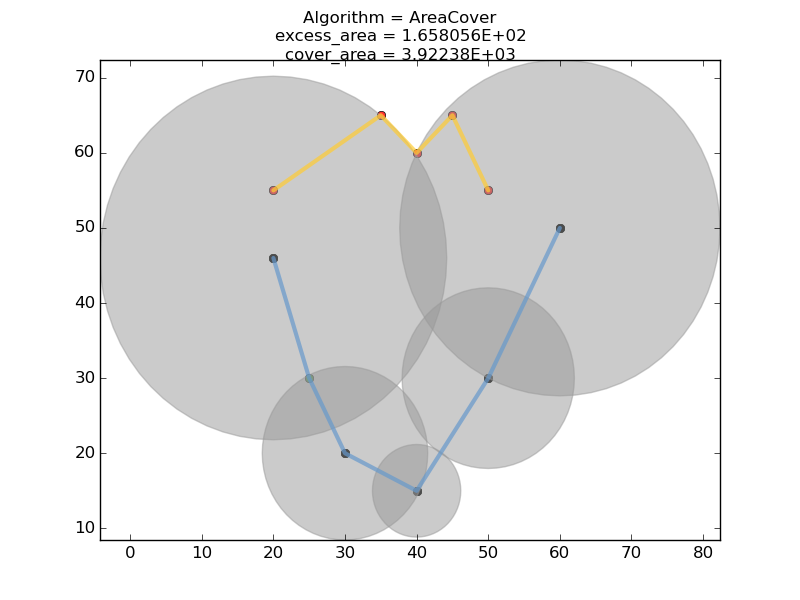
\includegraphics{/home/mranga/circle-cover/figures/estuary_areacover}

The detection\_coverage curves are depicted pictorially as follows:

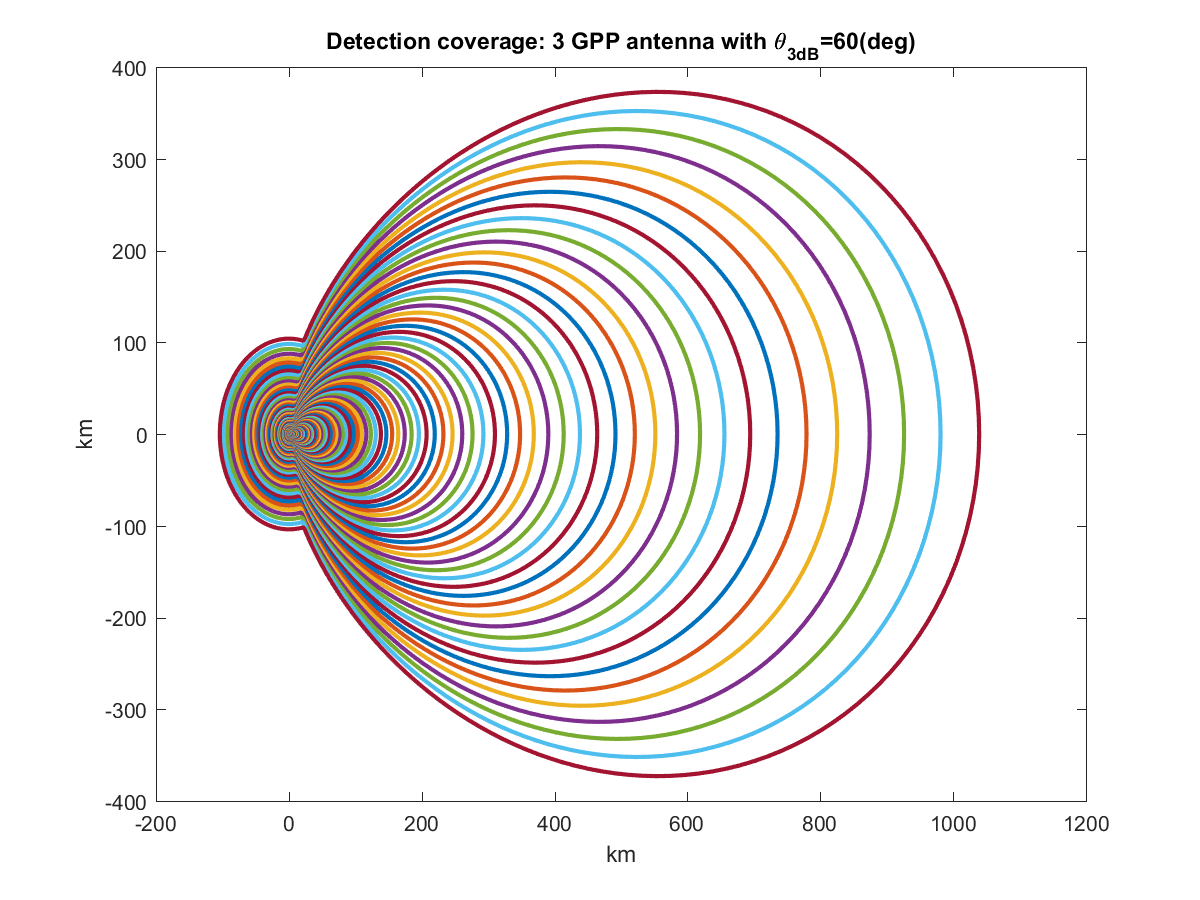
\includegraphics{/home/mranga/circle-cover/figures/DetectionCoverage_60deg}

After overlaying the detection coverage curves on the circle\_cover
and overlaying, we get the following result. Note that small regions
are uncovered because we eliminate lobes that cover less than threshold
points on our interference\_set :

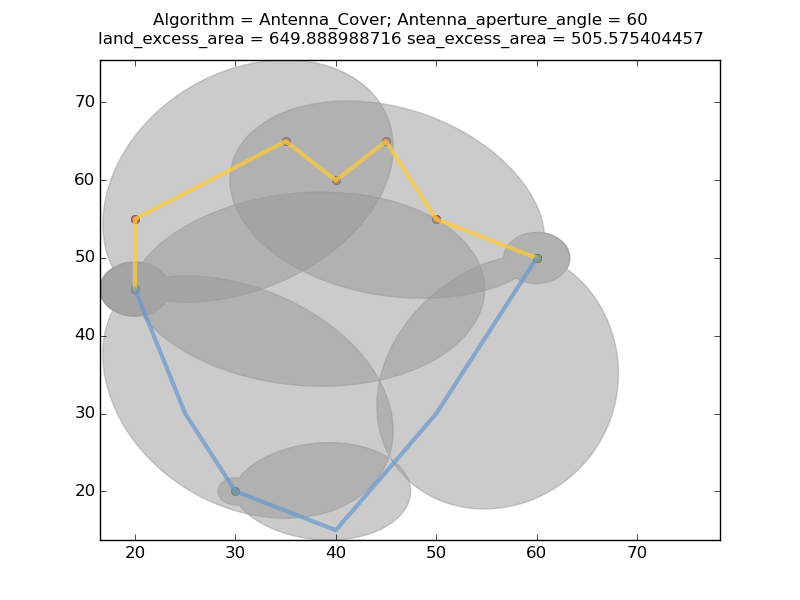
\includegraphics{/home/mranga/circle-cover/figures/estuary_antenna_60}

After applying simulated annealing on the figure above, we get:

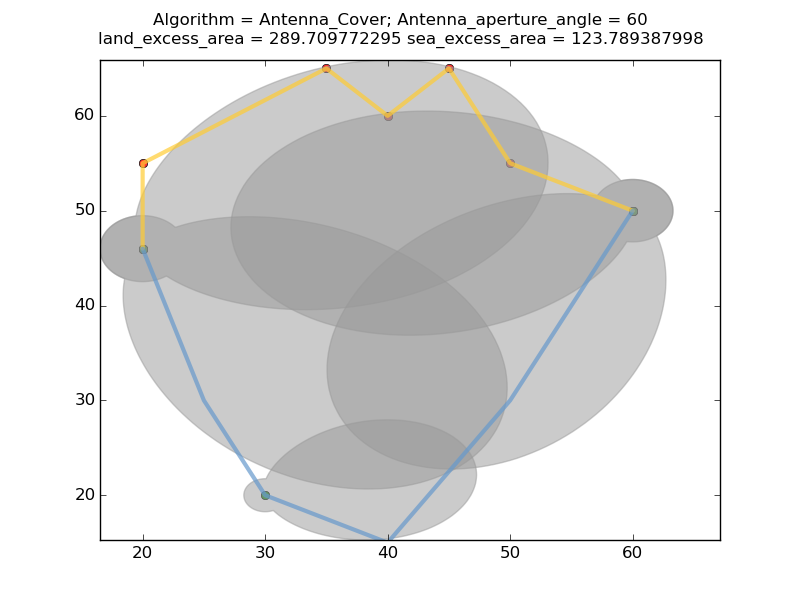
\includegraphics{/home/mranga/circle-cover/figures/estuaryanneal_antenna_60}
\end{document}
